\documentclass[submission,copyright,creativecommons]{eptcs}
\providecommand{\event}{ML 2014}

\usepackage{graphicx}
\usepackage{xcolor}
\usepackage[fleqn]{amsmath}
\usepackage[hang,flushmargin]{footmisc} 
\usepackage{graphics} 
%\usepackage{breakurl}

% =================================================================================================

\newcommand{\langl}{\begin{picture}(4.5,7)
\put(1.1,2.5){\rotatebox{60}{\line(1,0){5.5}}}
\put(1.1,2.5){\rotatebox{300}{\line(1,0){5.5}}}
\end{picture}}
\newcommand{\rangl}{\begin{picture}(4.5,7)
\put(.9,2.5){\rotatebox{120}{\line(1,0){5.5}}}
\put(.9,2.5){\rotatebox{240}{\line(1,0){5.5}}}
\end{picture}}

\newcommand{\lang}{\begin{picture}(5,7)
\put(1.1,2.5){\rotatebox{45}{\line(1,0){6.0}}}
\put(1.1,2.5){\rotatebox{315}{\line(1,0){6.0}}}
\end{picture}}
\newcommand{\rang}{\begin{picture}(5,7)
\put(.1,2.5){\rotatebox{135}{\line(1,0){6.0}}}
\put(.1,2.5){\rotatebox{225}{\line(1,0){6.0}}}
\end{picture}} 

\mathindent=1em

\definecolor{cmtclr}{rgb}{0.0,0.6,0.0}
\definecolor{kvdclr}{rgb}{0.0,0.0,0.6}
\definecolor{strclr}{rgb}{0.5,0.1,0.0}
\definecolor{prepclr}{rgb}{0.0,0.0,0.0}

\newcommand{\ignp}{\_\kern-.5ex\_\kern-.5ex\_ }
\newcommand{\kvd}[1]{\textnormal{\textcolor{kvdclr}{\sffamily #1}}}
\newcommand{\str}[1]{\textnormal{\textcolor{strclr}{\ttfamily "#1"}}}
\newcommand{\ident}[1]{\textnormal{\sffamily #1}}
\newcommand{\lident}[1]{\textnormal{\sffamily 
  \`{}\hspace{-0.25em}\`{}\hspace{-0.1em}#1\`{}\hspace{-0.25em}\`{}}}
\newcommand{\cmt}[1]{\textit{\sffamily\textcolor{cmtclr}{#1}}}
\newcommand{\narrow}[1]{\hspace{-0.75em} #1 \hspace{-1.25em}~}

% =================================================================================================

\title{In the Age of Web:\\
  \textnormal{\LARGE Typed Functional-First Programming Revisited}}

\author{Tomas Petricek
\institute{University of Cambridge, UK}
\email{tomas@tomasp.net}
\and
Don Syme
\institute{Microsoft Research Cambridge, UK}
\email{don.syme@microsoft.com}
}
\def\titlerunning{In the Age of Web: Typed Functional-First Programming Revisited}
\def\authorrunning{T. Petricek, D. Syme}
\begin{document}
\maketitle

% =================================================================================================

\begin{abstract}
% What is the problem
Most programming languages were designed before the age of web.
% Why is this a problem
This matters because the web changes many assumptions that typed functional language designers take 
for granted. For example, programs do not run in a closed word, but must instead interact with 
(changing and likely unreliable) services and data sources, communication is often asynchronous 
or event-driven, and programs need to interoperate with untyped environments.

% What is my solution
In this paper, we present how F\# language and libraries face the challenges posed by the web.
Technically, this comprises using \emph{type providers} for integration with external information 
sources and for integration with untyped programming environments, using \emph{lightweight 
meta-programming} for targetting JavaScript and \emph{computation expressions} for writing 
asynchronous code.

% Why does the solution matter
In this inquiry, the holistic perspective is more important than each of the features in isolation.
We use a practical case study as a starting point and look how F\# language and libraries approach 
the challenges posed by the web. The specific lessons learned are perhaps less interesting than 
our attempt to uncover hidden assumptions that no longer hold in the age of web.
\end{abstract}

% =================================================================================================

\section{Introduction}

Among the ML family of languages, F\# often takes a pragmatic approach and emphasizes ease of use
and the ability to integrate with its execution environments\footnote{Historically, this applied 
to the .NET runtime, but the same applies to integrating with JavaScript in the web context.} over 
other aspects of language design. If you use the F\# langage as ML, you get most of the good 
well-known properties of ML\footnote{For example, F\# does not require type annotations when used 
as ML, but requires them when used with .NET objects.}. However, F\# leaves enough \emph{holes} that
let you use it \emph{not} as ML. This is the space that we explore in this paper.

This additional flexibility makes it possible to use F\# in ways that break the common assumptions
that are often taken for granted in languages such as ML and Haskell\footnote{In a way, we are trying
to uncover the hidden assumptions of the functional programming \emph{research programme} that are
normally ``\emph{rendered unfalsifiable by the methodological decisions of its protagonists}.'' 
(Lakatos \cite{philosophy-lakatos} as quoted by Chalmers \cite{philosophy-thing})}. The focus on 
the web directs our inquiry and provides an angle for reconsidering such assumptions. 

Perhaps the most remarkable assumption is the idea that programs fundamentally operate in a closed
world. Although we have learned how to perform FFI and I/O \cite{haskell-ffi,haskell-imperative},
those are treated as dealing with the ``dirty real world''. For a practical solution, we argue that
we need to go much further, but deeper integration with (untyped) JavaScript libraries and (evolving) 
services inevitably breaks strict type safety requirements.

We do not claim that the F\# approach is the only possible. Rather, this paper should be seen
as a programming language experiment \cite{philosophy-pl} or an empirical observation of the 
approach used by the F\# community. We aim to provide an intriguing exploration of hidden assumptions 
and present what can be achieved using a combination of F\# features. We do so by starting with 
a simple, yet real-world problem and then exploring a solution. More specifically, the contributions 
of this position paper are:

\begin{itemize}
\item We present a case study (Section~\ref{sec:case}) showing how a combination of numerous
  F\# language features can be used for the development of modern web applications. This
  is not a toy demonstration, but an example of how F\# is used in the industry.

\item We discuss how type providers make it possible to access external information sources
  in web applications (Section~\ref{sec:tp-data}) and integration with (untyped) programming
  environments such as the JavaScript ecosystem (Section~\ref{sec:tp-lang}). 

\item We show how F\# approaches the problem of compilation to JavaScript using a library 
  called FunScript (Section~\ref{sec:js-meta}), outlining important practical concerns such as 
  interoperability (Section~\ref{sec:js-lib}) and asynchronous execution (Section~\ref{sec:js-async}).

\item Throughout the paper, we discuss how the age of the web breaks the assumptions commonly 
  taken as granted in typed functional programming. We revisit the notion of type safety
  in the context of web (Section~\ref{sec:tp-relative}) and the notion of fixed language 
  semantics (Section~\ref{sec:js-relative}).
\end{itemize}

\noindent
In the first part of the paper (Section~\ref{sec:case}), we present a case study of using 
F\# for web development. The rest of the paper (Section~\ref{sec:tp} and \ref{sec:js}) discusses 
the arising issues in more depth. The source code and running demo for the case study is available 
at: \url{http://funscript.info/samples/worldbank}

% =================================================================================================

\section{Case Study: Web-based data analytics}
\label{sec:case}
In this case study, we develop a web application shown in Figure~\ref{fig:wb}, which lets the
user compare university enrolment in a number of selected countries and regions around the world. 
The resulting application runs on the client-side (as JavaScript) and fetches data dynamically 
from the World Bank \cite{data-wb-schter}.

The application is an example of a web page that could be built in the context of data journalism 
\cite{dj-handbook}. As such, it is relatively simple, works with just a single data source and 
uses a concrete indicator and a hard-coded list of countries \emph{i.e.}~to illustrate a point 
made in an accompanying article.

% -------------------------------------------------------------------------------------------------

\subsection{Accessing World Bank data with type providers}

To access the university enrollment information, we first obtain a list of countries using the 
World Bank type provider from the F\# Data library \cite{fsharp-data}. The type provider exposes 
the individual countries as members of an object (the notation \lident{Country Name} is used for 
identifiers with spaces):
%
\begin{equation*}
\begin{array}{l}
 \kvd{type}~\ident{WorldBank}~=~\ident{WorldBankData}\langl\ident{Asynchronous}=\kvd{true}\rangl
 \\[0.5em]
 \kvd{let}~\ident{data}~=~\ident{WorldBank.GetDataContext}() \\
 \kvd{let}~\ident{countries}~= \\
 \quad~\lbrack~~ \ident{data.Countries.}\lident{European Union} \\
 \qquad   \ident{data.Countries.}\lident{Czech Republic} \\
 \qquad   \ident{data.Countries.}\lident{United Kingdom} \\
 \qquad   \ident{data.Countries.}\lident{United States} ~\rbrack 
\end{array}
\end{equation*}
%
The type provider connects to the World Bank and obtains a lisf of countries at 
\emph{compile-time} and at \emph{edit-time} (when using auto-completion in an editor).
This means that the list is always up-to-date and we get a compile time error when accessing 
a country that no longer exists (a property discussed in Section~\ref{sec:tp-data}).

On the first line, we provide a static parameter \ident{Asynchronous}. Static parameters are 
resolved at compile-time (or edit-time). Here, we specify that the exposed types for accessing 
information should support only non-blocking functions. This is necessary for a web-based 
application, because JavaScript only supports non-blocking calls (using callbacks) to fetch the data. 

% =================================================================================================

\begin{figure}[!t]
\hspace{3em} 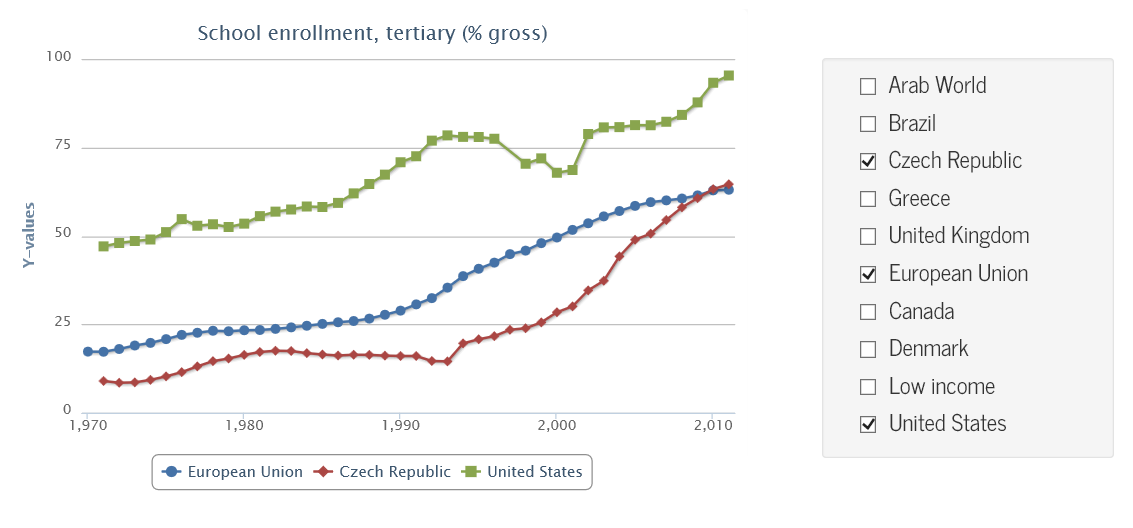
\includegraphics[width=35em]{worldbank.png}
\caption{Case study -- web application for comparing university enrollment in the world}
\label{fig:wb}
\end{figure}

% =================================================================================================

\subsection{Interoperating with JavaScript libraries}
To run the sample application on the client-side we use FunScript \cite{fsharp-funscript}, which 
is a library that translates F\# code to JavaScript (Section~\ref{sec:js}). Aside from 
running as JavaScript, we also want to use standard JavaScript libraries, including jQuery for DOM 
manipulation and Highcharts for charting. FunScript comes with a type provider that imports 
TypeScript \cite{ms-typescript} definitions for JavaScript libraries:
%
\begin{equation*}
\begin{array}{lll}
 \kvd{type}~\ident{j}~&\narrow{=}&~\ident{TypeScript}\langl\str{jquery.d.ts}\rangl \\
 \kvd{type}~\ident{h}~&\narrow{=}&~\ident{TypeScript}\langl\str{highcharts.d.ts}\rangl \\
\end{array}
\end{equation*}
%
The \textcolor{strclr}{\ttfamily d.ts} files are type annotations created for the TypeScript language.
Here, the type provider mechanism lets us leverage an existing effort for annotating common JavaScript 
libraries. The type provider analyses those definitions and maps them into F\# types named \ident{j} and 
\ident{h} that contain statically typed functions for calling the JavaScript libraries (we will use
them shortly). The file names are static parameters (same as \ident{Asynchronous} earlier) and are 
statically resolved and accessed at compile-time or edit-time.

Importing types for JavaScript libraries into the F\# type system has interesting implications, 
because the TypeScript language does not have the traditional type safety property \cite{ms-safets}.
We return to this topic in Section~\ref{sec:tp-lang}. Next, we generate checkboxes that appear on the 
right in Figure~\ref{fig:wb}:
%
\begin{equation*}
\begin{array}{lll}
 \kvd{let}~\ident{jQuery}~\ident{command}~=~\ident{j.jQuery.Invoke}(\ident{command}) 
 \\[0.5em]
 \kvd{let}~\ident{infos}~=~\ident{countries}~|\rang~\ident{List.map}~(\kvd{fun}~\ident{country}~\rightarrow \\
 \quad \kvd{let}~\ident{inp}~=~\ident{jQuery}(\str{<input>})\ident{.attr}(\str{type}, \str{checkbox}) \\
 \quad \ident{jQuery}(\str{\#panel})\ident{.append}(\ident{inp})\ident{.append}(\ident{country.Name}) \\
 \quad \ident{country.Name}, \ident{country.Indicators}, \ident{el}) \\
\end{array}
\end{equation*}
%
To manipulate the DOM (Document Object Model), we are using the jQuery library in a way that is
very similar to code that one would write in JavaScript. We define a helper function \ident{jQuery}
(hiding some of the complexities of the mapping) and use it to create the \str{<input>} element and
specify its attributes. Note that members like \ident{append} and \ident{attr} are standard 
jQuery patterns. The compiler sees them as ordinary object members. When writing code using F\# editors
based on the F\# Compiler Serivce \cite{fsharp-fcs}, they also appear in the auto-complete list.

Although the jQuery library is not perfect, it is a de facto standard in web development. The 
FunScript type provider makes it possible to integrate with it painlessly without explicitly 
specifying any FFI interface and without manual wrapping (see also Section~\ref{sec:js-lib}). 

Note that we use a standard F\# function \ident{List.map} to iterate over the countries. This has 
a side-effect of creating the HTML elements, but it also returns a new list. The result is a list 
of $\ident{string}\ast\ident{Indicators}\ast\ident{jQuery}$ values representing the country name,
its indicators (for accessing the World Bank data) and the created DOM object representing the
checkbox.

% -------------------------------------------------------------------------------------------------

\subsection{Loading data and updating the user interface}

The main part of the sample program is a function \ident{render} that asynchronously fetches 
data for selected countries and generates a chart. To keep the code simple, we iterate over the 
\ident{infos} list from the previous section and load data for countries one by one:
%
\begin{equation*}
\begin{array}{lll}
 \kvd{let}~\ident{render}~()~=~\ident{async}~\{ \\
 \quad \kvd{let}~\ident{head}~=~\str{School enrollment, tertiary (\% gross)} \\
 \quad \kvd{let}~\ident{o}~=~\ident{h.HighchartsOptions}() \\
 \quad \ident{o.chart} \leftarrow \ident{h.HighchartsChartOptions}(\ident{renderTo}=\str{plc}) \\
 \quad \ident{o.title} \leftarrow \ident{h.HighchartsTitleOptions}(\ident{text}~=~\ident{head}) \\
 \quad \ident{o.series} \leftarrow \lbrack| ~ |\rbrack
 \\[0.5em]   
 \quad \kvd{for}~\ident{name},~\ident{ind},~\ident{check}~\kvd{in}~\ident{infos}~\kvd{do}\\
 \qquad   \kvd{if}~\ident{unbox}\langl \ident{bool} \rangl~(\ident{check.is}(\str{:checked}))~\kvd{then} \\
 \qquad\quad     \kvd{let!}~\ident{v}~=~\ident{ind.}\lident{School enrollment, tertiary (\% gross)} \\
 \qquad\quad     \kvd{let}~\ident{data}~=~\ident{vals}~
                   |\rang~\ident{Seq.map}~(\kvd{fun}~(\ident{k}, \ident{v})~\rightarrow \lbrack|~\ident{number~k};~\ident{number~v} ~|\rbrack)~
                   |\rang~\ident{Array.ofSeq} \\
 \qquad\quad     \ident{opts.series.push}(\ident{h.HighchartsSeriesOptions}(\ident{data}, \ident{name})) ~\}
\end{array}
\end{equation*}
%
Although the function looks like ordinary code, it is wrapped in the $\ident{async}~\{\ldots\}$ 
block, which is an F\# computation expression \cite{fsharp-zoo}. The F\# compiler performs 
de-sugaring similar to the CPS transformation and interprets keywods such as \kvd{let!} and 
\kvd{for} using special operations (monadic bind and other). The \ident{async} identifier 
determines that we are writing asynchronous workflow \cite{fsharp-async} that makes it 
possible to include non-blocking calls in the block.

Here, the non-blocking call is done when accessing the \lident{School enrollment, tertiary (\% gross)} 
indicator using the \kvd{let!} keyword. The indicator is a member (with a name wrapped in 
back-ticks to allow spaces) exposed as an asynchronous computation by the World Bank type provider.
The rest of the code is mostly dealing with the DOM and the Highcharts library using the API 
imported by FunScript -- we iterate over all checkboxes and generate a new chart series for each 
checked country. 

Two notable points here are that \ident{async} translated to JavaScript is restricted to a single 
thread, which is not the case for ordinary F\# code (Section~\ref{sec:js-async}) and that the 
\ident{HighchartOptions} object preserves some of the underlying JavaScript semantics 
(Section~\ref{sec:js-lib}). Finally, the last part of the example code registers event handlers that 
redraw the chart when checkbox is clicked:
%
\begin{equation*}
\begin{array}{lll}
 \kvd{for}~\ignp, \ignp,~\ident{check}~\kvd{in}~\ident{infos}~\kvd{do} \\
 \quad \ident{check.click}(\kvd{fun}~\ignp~\rightarrow \ident{Async.StartImmediate}(\ident{render}()))
\end{array}
\end{equation*}
%
The \ident{click} operation (exposed by jQuery) takes a function that should be called when the 
event occurs. Calling it is a side-effectful operation that registers the handler. As \ident{render} 
is an asynchronous operation, we invoke it using the \ident{StartImmediate} primitive from the 
F\# library, which starts the computation without waiting for the result (the only way to start
a non-blocking operation in JavaScript).

% -------------------------------------------------------------------------------------------------

\subsection{Larning from the case study}

The case study shows that we can develop a simple interactive data visualization (that could
be built, for example, by data journalists) in less than 30 lines of F\# code. The code uses 
many typical functional patterns (lists, first-class functions, data types), but also uses features
that are more specific to F\# (type providers, objects, computation expressions). 

Before analysing the interesting aspects of this case study, we briefly review the points that we 
find appealing and points that many would find unappealing or, at least, peculiar. First, the 
appealing points:

\begin{itemize}
\item The ML approach to types and type inference can be extended from (closed-world) data types 
  to (open-world) types for rich information sources such as World Bank. The sample code is 
  fully statically typed without explicit type annotations. Critically, types are also used for 
  exploratory programming when finding indicators using auto-complete in an editor.

\item The case study demonstrates that core ML programming style can be used in the context of
  client-side (JavaScript) web development. We used functional lists, standard higher-order 
  functions such as \ident{List.map} in much the same way as when writing ordinary F\#.

\item In addition to standard functional constructs, we were also able to reuse F\# asynchronous
  workflows to write non-blocking code that requests data from a web service (World Bank), 
  rather than using error-prone explicit callbacks that are common in JavaScript.

\item Finally, we were able to painlessly call Highcharts and jQuery. No explicit wrapping or 
  importing of individual functions and types was necessary. Moreover, despite the differences between 
  the F\# and JavaScript object model, the code is close to idiomatic F\#.
\end{itemize}

\noindent
Now, the following list looks at the aspects that appear unappealing or peculiar, especially when 
coming from the traditional functional programming background:

\begin{itemize}
\item The World Bank type provider lifts information about countries to the type level. As a result,
  we can easily write $\ident{data.Countries.}\lident{Czech Republic}$, but if Czech Republic is
  removed from the World Bank (and becomes Czechoslovakia again), the code will no longer compile
  (Section~\ref{sec:tp-data}).

\item The TypeScript language is unsound due to covariant generics \cite{ms-safets}. Thus
  importing types from TypeScript definitions introduces a potential unsoundness into the F\# 
  code (Section~\ref{sec:tp-lang}).

\item When compiling F\# to JavaScript, the FunScript library does not fully preserve the 
  semantics of F\#. For example, numerical types behave as in JavaScript (Section~\ref{sec:js-meta})
  and asynchronous workflows run on a single thread (Section~\ref{sec:js-async}).
\end{itemize}

\noindent
The most notable observation about the above points is that there is often both a positive and
a negative side: we can nicely access World Bank data, but it affects soundness properties;
we can interoperate with JavaScript libraries, but we can not fully hide undesirable JavaScript 
behaviours.

The aim of this paper is not to make value judgements and argue what is better. Using the case
study as a basis, we claim that the outlined approach is \emph{one possible} and that it
\emph{works in practice}. In the rest of the paper, we give more details about the most important 
aspects of the approach and discuss alternatives`'.

% =================================================================================================

\section{Type providers}
\label{sec:tp}
a \\
b \\
c \\
~

\subsection{Integrating data}
\label{sec:tp-data}

~

\subsection{Integrating languages}
\label{sec:tp-lang}

~

\subsection{Relativized type safety}
\label{sec:tp-relative}

~

% =================================================================================================

\section{Compiling to JavaScript}
\label{sec:js}

~

\subsection{Quotations}
\label{sec:js-meta}

We have been doing this for long. You could use compiler backend or meta-programming.
For JS, backend is perhaps better. For SQL, Freebase, CUDA, ... meta-programming is good.

This is never going to work fully -- there are different exception mechanisms, different
numbers, different casts (for example, unbox)


\subsection{Libraries}
\label{sec:js-lib}

We could ignore all JS libraries and reimplement everything (or run every Hackage library).
This works for some scenarios, but not for the case study covered here.
You need to have access to standard JS libraries.

This brings challenges though -- because the libraries are not F\# libraries.
(for example, we have to initialize the array of series)

\subsection{Async}
\label{sec:js-async}

JavaScript async is single-threaded. Should we have ``js-async''? No, that would be mess,
accept that the semantics is relativized.

\subsection{Relativized semantics}
\label{sec:js-relative}

~
% =================================================================================================

\section{Conclusions and Future Work}

\cite{websharper-piglets} \cite{websharper-guis}

\subsection{Big Picture}
Is there a grand theory? No!

Perhaps we could claim one, but it isnt there [Feyerabend] -- and that is the point 
(leave holes).

\subsection{Conclusions}

% =================================================================================================

\nocite{*}
\bibliographystyle{eptcs}
\bibliography{generic}
\end{document}


